%\documentclass[twocolumn]{article} for when it needs to be two columns
\documentclass{article}
\usepackage{fullpage}
\usepackage{indentfirst}
\usepackage{amsmath}
\usepackage{amsfonts}
\usepackage{array}
\usepackage{tipa}
\usepackage{tikz}
\usepackage{tikz-qtree}
\usetikzlibrary{matrix, arrows, automata}
\usepackage{gb4e}
\noautomath
\usepackage{verbatim}
\newcommand{\Y}{$\checkmark$}
\newcommand{\N}{\ding{55}}
\newcommand{\R}{$\Rightarrow$}
\newcommand\myeq{\mathrel{\stackrel{\makebox[0pt]{\mbox{\normalfont\tiny def}}}{=}}}
\title{Revisions, New GM, and Zhenhai Transductions}
\author{Chris Oakden}
\begin{document}
\maketitle
There are four goals for this writeup:
\begin{itemize}
	\item Offer general statements about the primitives of the Yip and Bao models, axioms about their representation
	\item Revise the Zhenhai I/O transduction on the Bao model
	\item Propose general transductions between the models
	\item Create a transduction between the models on the Zhenhai data
\end{itemize}
\section{General Statements}
We begin by offering some general statements about Yip's and Bao's models respectively.\par
Elements in Yip's model are labeled with three types of unary predicates: the syllable TBU predicate $P_{\sigma}$, register node $P_{rf}$ predicates, and terminal tonal node $P_{cf}$ predicates. Register and contour nodes come in two varieties:
\begin{equation} \label{registerandcontour}
\begin{aligned}
P_{rf}&\myeq P_{+u}, P_{-u} \\
P_{cf}&\myeq P_{l}, P_{h}
\end{aligned}
\end{equation}
 These correspond to upper and lower register, and High and Low tones respectively. Within a particular syllable, there is at most one syllable TBU node, one register node, and up to two terminal tonal nodes. Tones can be either level (either one `l' or one `h' terminal node) or contour (`h+l' for falling, `l+h' for rising). No other terminal tonal node combinations are possible. \par
Within a syllable, the TBU node is the input of a binary function $\alpha(x)=y$. The output of this function is the register node.
\begin{equation}
\alpha(x)=y\myeq P_{\sigma}(x)\land P_{rf}(y)
\end{equation}
This function describes the association relation between a tautosyllabic TBU and a tonal root. Association holds between no other nodes in the model (including nodes in heterosyllabic syllables), nor is it reflexive. \par
The internal structure of the tone is defined by the binary function $\delta(x)=y$. This function takes the dominated element and yields its dominator. In Yip's model, terminal tonal nodes are dominated by the register node within the same syllable.
\begin{equation}
\delta(x)=y\myeq P_{cf}(x)\land P_{rf}(y)
\end{equation}
The dominance function is true for no other elements in the model (including in heterosyllabic syllables), nor is it reflexive. \par
Order is imposed on the structure via the successor function $succ(x)$. This function defines order within elements \emph{of the same type}, that is, terminal tonal nodes within a syllable and across syllables, heterosyllabic syllable nodes, and heterosyllabic register nodes. The function is total, such that the final element in a domain is its own successor. Additionally, the successor function can be used to restrain association and dominance to single syllables, as below.
\begin{equation}
\begin{aligned}
\alpha(x)=y&\myeq P_{\sigma} \land P_{rf}(y) \land [\alpha(succ(x)) = succ(y)]\\
\delta(x)=y&\myeq P_{rf} \land P_{cf}(y) \land [\delta(succ(x)) = succ(y)\lor \delta(succ(succ(x))=succ(y)]\\
\end{aligned}
\end{equation} \par
The Yip model is thus:
\begin{center}
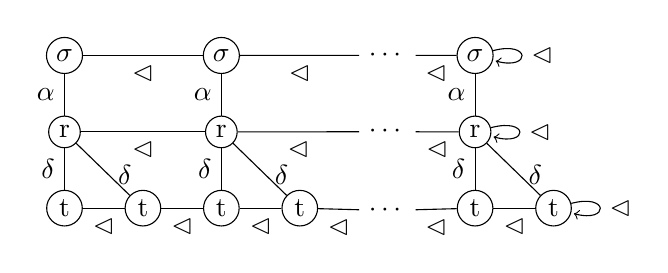
\begin{tikzpicture} [baseline = (x.base)]
\matrix (m) [matrix of nodes, column sep = 1.5em, row sep = 1.5em]{
\node[draw,circle, inner sep =2pt](x){$\sigma$}; & & \node[draw,circle, inner sep =2pt](x2){$\sigma$}; & & \node(x25){$\dotsb$}; & \node[draw,circle, inner sep =2pt](x3){$\sigma$};  \\
\node[draw,circle, inner sep =2pt](y){r}; & & \node[draw,circle, inner sep =2pt](y2){r}; & & \node(y25){$\dotsb$}; & \node[draw,circle, inner sep =2pt](y3){r};  \\
\node[draw,circle, inner sep =2pt](z){t}; & \node[draw,circle, inner sep =2pt](v){t}; & \node[draw,circle, inner sep =2pt](z2){t}; & \node[draw,circle, inner sep =2pt](v2){t}; & \node(z25){$\dotsb$}; & \node[draw,circle, inner sep =2pt](z3){t}; & \node[draw,circle, inner sep =2pt](v3){t};\\
};
\draw (x) -- (y) node[left, pos=.5]{$\alpha$};
\draw (z) -- (y) node[left, pos=.5]{$\delta$};
\draw (v) -- (y) node [right, pos =.4]{$\delta$};
\draw (x2) -- (y2) node[left, pos=.5]{$\alpha$};
\draw (z2) -- (y2) node[left, pos=.5]{$\delta$};
\draw (v2) -- (y2) node [right, pos =.4]{$\delta$};
\draw (x3) -- (y3) node[left, pos=.5]{$\alpha$};
\draw (z3) -- (y3) node[left, pos=.5]{$\delta$};
\draw (v3) -- (y3) node [right, pos =.4]{$\delta$};
\draw (x) -- (x2) node[below, pos=.5]{$\vartriangleleft$};
\draw (x2) -- (x25) node[below, pos=.5]{$\vartriangleleft$};
\draw (x25) -- (x3) node[below, pos=.5]{$\vartriangleleft$};
\draw (v) -- (z2) node[below, pos=.5]{$\vartriangleleft$};
\draw (v2) -- (z25) node[below, pos=.5]{$\vartriangleleft$};
\draw (z25) -- (z3) node[below, pos=.5]{$\vartriangleleft$};
\draw (z) -- (v) node[below, pos=.5]{$\vartriangleleft$};
\draw (z2) -- (v2) node[below, pos=.5]{$\vartriangleleft$};
\draw (z3) -- (v3) node[below, pos=.5]{$\vartriangleleft$};
\path (x3) edge [loop right, align = center] node{$\vartriangleleft$} (x3);
\path (v3) edge [loop right, align = center] node{$\vartriangleleft$} (v3);
\draw (y) -- (y2) node[below, pos=.5]{$\vartriangleleft$};
\draw (y2) -- (y25) node[below, pos=.5]{$\vartriangleleft$};
\draw (y25) -- (y3) node[below, pos=.5]{$\vartriangleleft$};
\path (y3) edge [loop right, align = center] node{$\vartriangleleft$} (y3);
\end{tikzpicture}
\end{center} \par
Bao's model is similar to Yip's model, with a few extensions and revisions. Two more unary predicates are necessary in addition to the original three (which are defined identically): the tonal root node `T' predicate $P_{T}$, and the contour node `c' predicate $P_{c}$. Within a single syllable, there is a maximum of one syllable node, one `T' node, one register node, one `c' node, and up to two terminal tonal nodes. Binary functions are modified such that association obtains between the syllable TBU and the `T' node, and a different set of dominance relations. The definitions below restrict dominance and association to tautosyllabic nodes.
\begin{equation}
\begin{aligned}
\alpha(x)=y&\myeq P_{\sigma}(x)\land P_{T}(y)\land[\alpha(succ(x))=succ(y)]\\
\delta(x)=y&\myeq \big[P_{rf}(x)\land P_{T}(y)\land[\delta(succ(x))=succ(y)]\big]\lor \\
&\quad \, \, \big[P_{c}(x)\land P_{T}(y)\land[\delta(succ(x))=succ(y)]\big]\lor \\
&\quad \, \, \big[P_{cf}(x)\land P_{c}(y)\land[\delta(succ(x))=succ(y)\lor \delta(succ(succ(x))=succ(y)]\big]\\
\end{aligned}
\end{equation}
These functions are true only under the definitions given above, and neither function is reflexive. \par
Much like the Yip model, the successor function in Bao's model is defined over elements of the same type. Note that no order is imposed between register and `c' nodes, in spite of the fact that they are sisters within the same syllable. The Bao model is thus:
\begin{center}
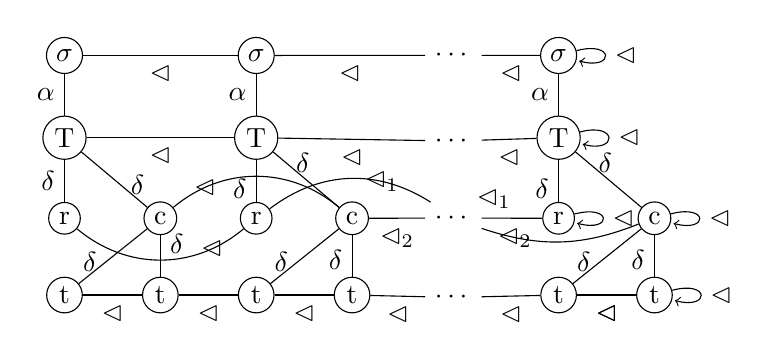
\begin{tikzpicture} [baseline = (x.base)]
\matrix (m) [matrix of nodes, column sep = 2em, row sep = 1.5em]{
\node[draw,circle, inner sep =2pt](x){$\sigma$}; & & \node[draw,circle, inner sep =2pt](x2){$\sigma$}; & & \node(x25){$\dotsb$}; & \node[draw,circle, inner sep =2pt](x3){$\sigma$};  \\
\node[draw,circle, inner sep =2pt](y){T}; & & \node[draw,circle, inner sep =2pt](y2){T}; & & \node(y25){$\dotsb$}; & \node[draw,circle, inner sep =2pt](y3){T};  \\
\node[draw,circle, inner sep =2pt](z){r}; & \node[draw,circle, inner sep =2pt](v){c}; & \node[draw,circle, inner sep =2pt](z2){r}; & \node[draw,circle, inner sep =2pt](v2){c}; &  \node(v25){$\dotsb$}; & \node[draw,circle, inner sep =2pt](z3){r}; & \node[draw,circle, inner sep =2pt](v3){c};\\
\node[draw,circle, inner sep =2pt](q){t}; & \node[draw,circle, inner sep =2pt](s){t}; & \node[draw,circle, inner sep =2pt](q2){t}; & \node[draw,circle, inner sep =2pt](s2){t}; &  \node(s25){$\dotsb$}; &  \node[draw,circle, inner sep =2pt](q3){t}; & \node[draw,circle, inner sep =2pt](s3){t}; \\
};
\draw (x) -- (y) node[left, pos=.5]{$\alpha$};
\draw (z) -- (y) node[left, pos=.5]{$\delta$};
\draw (v) -- (y) node [right, pos =.4]{$\delta$};
\draw (q) -- (v) node [left, pos=.4]{$\delta$};
\draw (s) -- (v) node [right, pos=.8]{$\delta$};
\draw (q) -- (s) node[below, pos=.5]{$\vartriangleleft$};
\draw (x2) -- (y2) node[left, pos=.5]{$\alpha$};
\draw (z2) -- (y2) node[left, pos=.3]{$\delta$};
\draw (v2) -- (y2) node [right, pos =.8]{$\delta$};
\draw (q2) -- (v2) node [left, pos=.4]{$\delta$};
\draw (s2) -- (v2) node [left, pos=.4]{$\delta$};
\draw (q2) -- (s2) node[below, pos=.5]{$\vartriangleleft$};
\draw (x3) -- (y3) node[left, pos=.5]{$\alpha$};
\draw (z3) -- (y3) node[left, pos=.3]{$\delta$};
\draw (v3) -- (y3) node [right, pos =.8]{$\delta$};
\draw (q3) -- (v3) node [left, pos=.4]{$\delta$};
\draw (s3) -- (v3) node [left, pos=.4]{$\delta$};
\draw (q3) -- (s3) node[below, pos=.5]{$\vartriangleleft$};
\draw (q3) -- (s3) node[below, pos=.5]{$\vartriangleleft$};
\draw (x) -- (x2) node[below, pos=.5]{$\vartriangleleft$};
\draw (x2) -- (x25) node[below, pos=.5]{$\vartriangleleft$};
\draw (x25) -- (x3) node[below, pos=.5]{$\vartriangleleft$};
\draw (s) -- (q2) node[below, pos=.5]{$\vartriangleleft$};
\draw (s2) -- (s25) node[below, pos=.5]{$\vartriangleleft$};
\draw (s25) -- (q3) node[below, pos=.5]{$\vartriangleleft$};
\path (z2) edge [bend left =35] node[pos=.7]{$\vartriangleleft_1$} (v25);
\draw (v2) -- (v25) node [below,pos=.5]{$\vartriangleleft_2$};
\draw (v25) -- (z3) node [above, pos=.2]{$\vartriangleleft_1$};
\path (v25) edge [bend right=20] node[pos=.2]{$\vartriangleleft_2$} (v3);
\path (x3) edge [loop right, align = center] node{$\vartriangleleft$} (x3);
\path (s3) edge [loop right, align = center] node{$\vartriangleleft$} (s3);
\draw (y) -- (y2) node[below, pos=.5]{$\vartriangleleft$};
\draw  (y2) -- (y25) node[below, pos=.5]{$\vartriangleleft$};
\draw  (y25) -- (y3) node[below, pos=.5]{$\vartriangleleft$};
\path (y3) edge [loop right, align = center] node{$\vartriangleleft$} (y3);
\path (v) edge [bend left = 40] node[pos=.2]{$\vartriangleleft$} (v2);
\path (v3) edge [loop right, align = center] node{$\vartriangleleft$} (v3);
\path (z) edge [bend right = 40] node[pos=.8]{$\vartriangleleft$} (z2);
\path (z3) edge [loop right, align = center] node{$\vartriangleleft$} (z3);
\end{tikzpicture}
\end{center}
\section{Revisions to Bao Zhenhai I/O Transduction}
In this section, we revise the I/O transduction for the Zhenhai contour shift pattern using the Bao model. This transduction adopts the second alternative analysis from the previous writeup, that is, the analysis where the de-linked `c' node from the second syllable is `deleted' from the output. Improvements on the first pass at this transduction include new definitions for unary predicates, a new definition of the dominance function, as well as the introduction of a second copy set to account for the `default l rule' where the `c' node of the first syllable associates to a default terminal `l' node. Since the `c' node in the first copy set contains the l-h contour which associates to the second syllable, this `c' node will come from the second copy set. Consider the transduction below:
\begin{equation}
\begin{aligned}
P_{\sigma}^{1}(x)&\myeq P_{\sigma}(x) & P_{\sigma}^{2}(x)&\myeq \mathtt{False}  \\
P_{T}^{1}(x)&\myeq P_{T}(x) & P_{T}^{2}(x)&\myeq \mathtt{False} \\
P_{rf}^{1}(x)&\myeq P_{rf}(x) & P_{rf}^{2}(x)&\myeq \mathtt{False} \\
P_{c}^{1}(x)&\myeq P_{c}(x) \land \neg last(x) & P_{c}^{2}(x)&\myeq P_{c}(x) \land \neg last(x) \\
P_{h}^{1}(x)&\myeq P_{h}(x)\land \neg last(\delta(x)) & P_{h}^{2}(x)&\myeq \mathtt{False} \\
P_{l}^{1}(x)&\myeq P_{l}(x) \land \neg last(\delta(x)) & P_{l}^{2}(x)&\myeq P_{l}(x) \land \neg last(\delta(x)) \\
\alpha^{1,1}(x)=y&\myeq \alpha(x)=y & \alpha^{1,2}(x)=y&\myeq \mathtt{False} \\
\alpha^{2,1}(x)=y&\myeq \mathtt{False} & \alpha^{2,2}(x)=y&\myeq \mathtt{False} \\
\delta^{1,1}(x)=y&\myeq \Big[P_{rf}(x)\land P_{T}(y)\land  & \delta^{1,2}(x)=y&\myeq \mathtt{False} \\
&\quad \, \, [\delta(succ(x))=succ(y)]\Big] \lor \\
&\quad \, \, \Big[P_{cf}(x)\land P_{c}(y)\land \\
&\quad \, \, \neg last(\delta(x))\land \neg last(y)\Big]\lor \\
&\quad \, \, \Big[P_{c}(x)\land P_{T}(y)\land \\
&\quad \, \, \neg last(x)\land last(y)\Big] \\
\delta^{2,1}(x)=y&\myeq P_{c}(x)\land P_{T}(y) \land  & \delta^{2,2}(x)=y&\myeq P_{l}(x)\land P_{c}(y)\land  \\
&\quad \, \, \neg last(x)\land\neg last(y) & &\quad\,\, last(\delta(x))\land \neg last(y) \\
\end{aligned}
\end{equation}
Here, the `c' node and its daughters from the first syllable only are produced (in the first copy set), effectively deleting the falling contour on the second syllable. A `c' node with a single `l' segment is produced in the second copy set to accommodate the default `l' rule. Association on the output form is identical to the input (that is, only defined from the first copy set to the first copy set). The definition of $\delta^{1,1}(x)=y$ preserves the relations between register and `T' nodes, while also shifting the `c' node from the first syllable to the second (``contour shift"). $\delta^{2,1}(x)=y$ associates the epenthesized `l' tone to the root node in the first syllable and $\delta^{2,2}(x)=y$ creates the internal structure of the epenthesized tone. 
The result is something like this:
\begin{center}
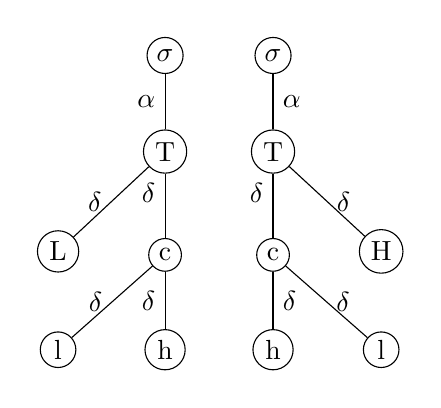
\begin{tikzpicture} [baseline = (y1.base)]
\matrix (m) [matrix of nodes, column sep = 2.3em, row sep = 2em]{
& \node[draw,circle, inner sep =2pt](x1){$\sigma$};  &  \node[draw,circle, inner sep =2pt](x2){$\sigma$};  \\
& \node[draw,circle, inner sep =2pt](y1){T}; &   \node[draw,circle, inner sep =2pt](y2){T}; \\
\node[draw,circle, inner sep =2pt](z1){L}; & \node[draw,circle, inner sep =2pt](z2){c}; &   \node[draw,circle, inner sep =2pt](z3){c}; & \node[draw,circle, inner sep =2pt](z4){H}; \\
\node[draw,circle, inner sep =2pt](t1){l}; & \node[draw,circle, inner sep =2pt](t2){h}; &  \node[draw,circle, inner sep =2pt](t3){h}; & \node[draw,circle, inner sep =2pt](t4){l}; \\
};
\draw (x1) -- (y1) node[left, pos=.5]{$\alpha$};
\draw (x2) -- (y2) node[right, pos=.5]{$\alpha$};
\draw (z1) -- (y1) node[left, pos=.5]{$\delta$};
\draw (z2) -- (y1) node[left, pos=.7]{$\delta$};
\draw (z3) -- (y2) node[left, pos=.7]{$\delta$};
\draw (z2) -- (t1) node[left, pos=.5]{$\delta$};
\draw (z2) -- (t2) node[left, pos=.5]{$\delta$};
\draw (y2) -- (z4) node[right, pos=.5]{$\delta$};
\draw (z3) -- (t3) node[right, pos=.5]{$\delta$};
\draw (z3) -- (t4) node[right, pos=.5]{$\delta$};
\end{tikzpicture}
\hspace{.5cm}
$\rightarrow$
\hspace{.5cm}
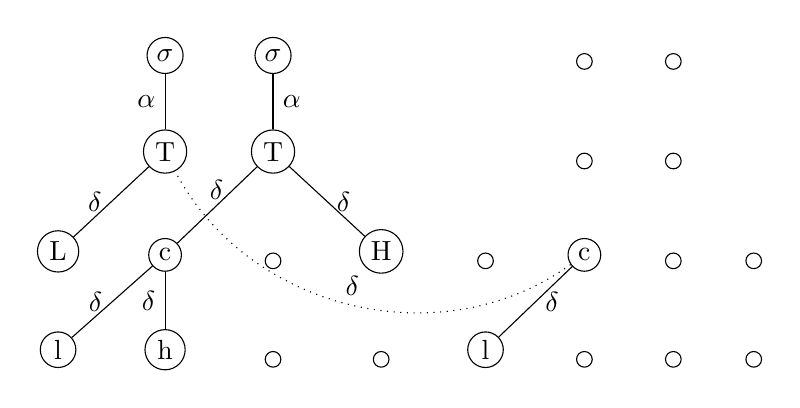
\begin{tikzpicture} [baseline = (y1.base)]
\matrix (m) [matrix of nodes, column sep = 2.3em, row sep = 2em]{
& \node[draw,circle, inner sep =2pt](x1){$\sigma$};  &  \node[draw,circle, inner sep =2pt](x2){$\sigma$}; & & & \node[draw,circle, inner sep =2pt](x3){\hspace{1em}}; & \node[draw,circle, inner sep =2pt](x4){\hspace{1em}}; \\
& \node[draw,circle, inner sep =2pt](y1){T}; &   \node[draw,circle, inner sep =2pt](y2){T}; & & & \node[draw,circle, inner sep =2pt](y3){\hspace{1em}};  & \node[draw,circle, inner sep =2pt](y4){\hspace{1em}};\\
\node[draw,circle, inner sep =2pt](z1){L}; & \node[draw,circle, inner sep =2pt](z2){c}; &   \node[draw,circle, inner sep =2pt](z3){\hspace{1em}}; & \node[draw,circle, inner sep =2pt](z4){H}; & \node[draw,circle, inner sep =2pt](z5){\hspace{1em}};  & \node[draw,circle, inner sep =2pt](z6){c}; & \node[draw,circle, inner sep =2pt](z7){\hspace{1em}}; & \node[draw,circle, inner sep =2pt](z8){\hspace{1em}};   \\
\node[draw,circle, inner sep =2pt](t1){l}; & \node[draw,circle, inner sep =2pt](t2){h}; &  \node[draw,circle, inner sep =2pt](t3){\hspace{1em}}; & \node[draw,circle, inner sep =2pt](t4){\hspace{1em}}; & \node[draw,circle, inner sep =2pt](t5){l};  & \node[draw,circle, inner sep =2pt](t6){\hspace{1em}}; & \node[draw,circle, inner sep =2pt](t7){\hspace{1em}}; & \node[draw,circle, inner sep =2pt](t8){\hspace{1em}}; \\
};
\draw (x1) -- (y1) node[left, pos=.5]{$\alpha$};
\draw (x2) -- (y2) node[right, pos=.5]{$\alpha$};
\draw (z1) -- (y1) node[left, pos=.5]{$\delta$};
\draw (z2) -- (y2) node[left, pos=.7]{$\delta$};
\draw (z2) -- (t1) node[left, pos=.5]{$\delta$};
\draw (z2) -- (t2) node[left, pos=.5]{$\delta$};
\draw (y2) -- (z4) node[right, pos=.5]{$\delta$};
\draw (t5) -- (z6) node [right, pos=.5]{$\delta$};
\path [dotted] (z6) edge [bend left = 49] node[above]{$\delta$} (y1);
\end{tikzpicture}
\hspace{.3cm}
\end{center}
\begin{comment}
or...
\begin{center}
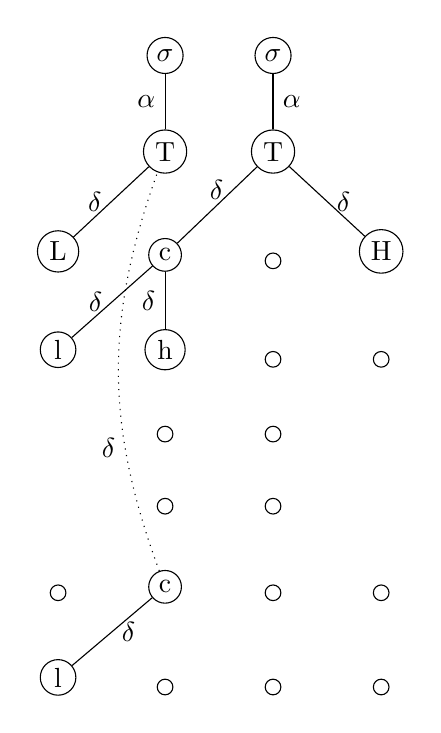
\begin{tikzpicture}[baseline = (x1.base)]
\matrix (m) [matrix of nodes, column sep = 2.3em, row sep = 2em]{
& \node[draw,circle, inner sep =2pt](x1){$\sigma$};  &  \node[draw,circle, inner sep =2pt](x2){$\sigma$}; \\
& \node[draw,circle, inner sep =2pt](y1){T}; &   \node[draw,circle, inner sep =2pt](y2){T}; \\
\node[draw,circle, inner sep =2pt](z1){L}; & \node[draw,circle, inner sep =2pt](z2){c}; &   \node[draw,circle, inner sep =2pt](z3){\hspace{1em}}; & \node[draw,circle, inner sep =2pt](z4){H}; \\
\node[draw,circle, inner sep =2pt](t1){l}; & \node[draw,circle, inner sep =2pt](t2){h}; &  \node[draw,circle, inner sep =2pt](t3){\hspace{1em}}; & \node[draw,circle, inner sep =2pt](t4){\hspace{1em}}; \\
& \node[draw,circle, inner sep =2pt](x3){\hspace{1em}}; & \node[draw,circle, inner sep =2pt](x4){\hspace{1em}}; \\
& \node[draw,circle, inner sep =2pt](y3){\hspace{1em}};  & \node[draw,circle, inner sep =2pt](y4){\hspace{1em}};\\
\node[draw,circle, inner sep =2pt](z5){\hspace{1em}};  & \node[draw,circle, inner sep =2pt](z6){c}; & \node[draw,circle, inner sep =2pt](z7){\hspace{1em}}; & \node[draw,circle, inner sep =2pt](z8){\hspace{1em}};   \\
\node[draw,circle, inner sep =2pt](t5){l};  & \node[draw,circle, inner sep =2pt](t6){\hspace{1em}}; & \node[draw,circle, inner sep =2pt](t7){\hspace{1em}}; & \node[draw,circle, inner sep =2pt](t8){\hspace{1em}}; \\
};
\draw (x1) -- (y1) node[left, pos=.5]{$\alpha$};
\draw (x2) -- (y2) node[right, pos=.5]{$\alpha$};
\draw (z1) -- (y1) node[left, pos=.5]{$\delta$};
\draw (z2) -- (y2) node[left, pos=.7]{$\delta$};
\draw (z2) -- (t1) node[left, pos=.5]{$\delta$};
\draw (z2) -- (t2) node[left, pos=.5]{$\delta$};
\draw (y2) -- (z4) node[right, pos=.5]{$\delta$};
\draw (t5) -- (z6) node [right, pos=.5]{$\delta$};
\path [dotted] (z6) edge [bend left = 20] node[left,pos=.3]{$\delta$} (y1);
\end{tikzpicture}
\end{center}
\end{comment}
One issue yet to be resolved is how the successor function is defined. The result we want is for all ordering relations to stay the same, but add an ordering where the `c' and terminal nodes in the first copy set (now dominated by the second `T' node) are the respective successors of the `c' and `l' nodes in the second copy set. I'm not sure how to do this. Is it possible that this ordering is inherited from the preserved ordering of the `T' nodes themselves? I will continue to work on this.
\section{General Transductions}
In an earlier writeup, we proposed general transductions between models. Here, we revise them to accommodate polysyllabic forms. Consider the general transduction from Bao's model to Yip's model.
\begin{equation}
\begin{aligned}
P^{\Gamma}_{\sigma}(x)&\myeq P_{\sigma}(x) \\
P^{\Gamma}_{rf}(x)&\myeq P_{T}(x) \\
P^{\Gamma}_{cf}(x)&\myeq P_{cf}(x) \\
\alpha^{\Gamma}(x)=y&\myeq P_{\sigma}(x)\land P_{t}(y)\land [\alpha(succ(x)) = succ(y)] \\
\delta^{\Gamma}(x)=y&\myeq P_{cf}(x)\land P_{T}(y) \land [\delta(succ(x))=succ(y) \lor \delta(succ(succ(x)))=succ(y)]\\
succ^{\Gamma}(x)&\myeq succ(x)
\end{aligned}
\end{equation}
This transduction captures the equivalency between Bao's T node and Yip's register node as the tonal root. Additionally, the definitions of association and dominance account for monosyllabic and polysyllabic structures. \par
Translating from the Yip model to the Bao model requires a transduction with a copy set of size two. Recall that in an earlier writeup, this strategy was also used to derive the structural similarities between the register node in Yip's model and both the `T' and `c' nodes in Bao's model. Working from that initial attempt, we can append the association and dominance functions to limit these relations to tautosyllabic nodes as we have done above. However, this will not work.
\begin{equation}
\begin{aligned}
P^1_{\sigma}(x) &\myeq P_{\sigma}(x) &  P^2_{\sigma}(x) &\myeq \mathtt{False} \\
P^1_{T}(x) &\myeq P_{rf}(x) &  P^2_{T}(x) &\myeq \mathtt{False} \\
P^1_{rf}(x) &\myeq \mathtt{False} &  P^2_{rf}(x) &\myeq P_{\sigma}(x) \\
P^1_{c}(x) &\myeq \mathtt{False} &  P^2_{c}(x) &\myeq P_{rf}(x) \\
P^1_{cf}(x) &\myeq \mathtt{False} &  P^2_{cf}(x) &\myeq P_{cf}(x) \\
\alpha^{1,1}(x)=y &\myeq P_{\sigma}(x)\land P_{rf}(y)\land  & \alpha^{1,2}(x)=y &\myeq \mathtt{False}  \\
&\quad \, \, [\alpha(succ(x))=succ(y)] \\
\alpha^{2,1}(x)=y &\myeq \mathtt{False} & \alpha^{2,2}(x)=y &\myeq \mathtt{False}  \\
\delta^{1,1}(x)=y &\myeq \mathtt{False} & \delta^{1,2}(x)=y &\myeq \mathtt{False}  \\
\delta^{2,1}(x)=y &\myeq\big[P_{\sigma}(x) \land P_{rf}(y) \land  & \delta^{2,2}(x)=y &\myeq P_{cf}(x)\land P_{rf}(y)\land \\
&\quad \, \, [\delta(succ(x))=succ(y)]\big]\lor & &\quad \, \, [\delta(succ(x))=succ(y)\lor  \\
&\quad \, \, \big[P_{rf}(x)\land P_{rf}(y)\land & & \quad \, \, \delta(succ(succ(x)))=succ(y)]\\
&\quad \, \, [\delta(succ(x))=succ(y)]\big] \\
\end{aligned}
\end{equation}
The problem here is in the part of the definitions of the dominance function that ensure that dominance only occurs within syllables and not between syllables. In defining unary predicates on the second copy set, we use structural positions that are not identical (or even equivalent) to the input. Specifically, we define the register node in the structural position of the syllable. We refer to the definition of $\delta(x)=y$ in the input structure along with $succ(x)$, but given the structural mismatches, sometimes those relations \emph{are not available} since they are not defined that way in the input structure. This is not an issue for the definition of $\delta^{2,2}(x)=y$, but it is for $\delta^{2,1}(x)=y$. There is no such definition of dominance between syllable and register in the input model (perhaps we can change it to $\alpha(succ(x)) = succ(y)$ since that relation does hold in the input structure), and certainly no definition of dominance between register nodes. I have yet to reach a satisfying solution to this problem, and will continue to work it out.
\section{Transductions between models: Zhenhai}
We have shown that we can perform transductions to translate from Bao's model to Yip's model and vice versa, and that the complexity of these transductions is QF. We have also shown that we can represent contour spreading in Zhenhai using Bao's model, in accordance with previous analyses. The data from Zhenhai are used as an example of a pattern which is impossible to represent in Yip's model. However, if there is some equivalency between the two (such that one can translate between them using simple logics), should there be processes that can be formalized in one model but not the other? \par
I have considered a number of approaches to doing a `transduction between the two models' on the Zhenhai data, but haven't stopped to think about what that actually means, and what the possibilities are. One is a transduction on a Zhenhai input from Bao's model to Yip's model. Another is the same, but on outputs. Neither would capture what is of interest to us, which is the \emph{process} itself. So, I will first attempt to model contour spreading with an I/O contour using Yip's model. This is presented in the transduction below:\footnote{I am abstracting away from the default rule for now. Suffice it to say that the default insertion of the `l' tone would proceed in the same way as for the Bao model in section 2: adding a second copy of a terminal tonal `l' node from the first syllable, and then defining domination from the second copy set to the first such that `l' in copy 2 is dominated by the low register node from copy 1.}
\begin{equation}
\begin{aligned}
P^{\tau}_{\sigma}(x)&\myeq P_{\sigma}(x) \\
P^{\tau}_{rf}(x)&\myeq P_{rf}(x) \\
P^{\tau}_{l}(x)&\myeq P_{l}(x)\land \neg last(\delta(x)) \\
P^{\tau}_{h}(x)&\myeq P_{h}(x)\land \neg last(\delta(x)) \\
\alpha^{\tau}(x)=y&\myeq \alpha(x)=y \\
\delta^{\tau}(x)=y&\myeq P_{cf}(x)\land P_{rf}(y) \land \neg last(\delta(x))\land last(y)
\end{aligned}
\end{equation}
The definitions are straightforward. The intuition here is to preserve only the `l' and 'h' tones (the rising contour) on the first syllable while deleting the tones from the second syllable. This is achieved by adding a second conjunct $\neg last(\delta(x))$ to the unary relations on terminal tonal nodes. Then, the dominance function is defined such that these tones are dominated by the register node on the final syllable. Note that this definition is similar to that proposed for the same transduction using Bao's model (both the version in this writeup and the previous version). 
\begin{center}
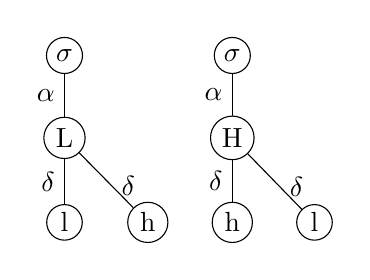
\begin{tikzpicture} [baseline = (y.base)]
\matrix (m) [matrix of nodes, column sep = 1.5em, row sep = 1.5em]{
\node[draw,circle, inner sep =2pt](x){$\sigma$}; & & \node[draw,circle, inner sep =2pt](x2){$\sigma$}; \\
\node[draw,circle, inner sep =2pt](y){L}; & & \node[draw,circle, inner sep =2pt](y2){H};  \\
\node[draw,circle, inner sep =2pt](z){l}; & \node[draw,circle, inner sep =2pt](v){h}; & \node[draw,circle, inner sep =2pt](z2){h}; & \node[draw,circle, inner sep =2pt](v2){l}; \\
};
\draw (x) -- (y) node[left, pos=.5]{$\alpha$};
\draw (z) -- (y) node[left, pos=.5]{$\delta$};
\draw (v) -- (y) node [right, pos =.4]{$\delta$};
\draw (x2) -- (y2) node[left, pos=.5]{$\alpha$};
\draw (z2) -- (y2) node[left, pos=.5]{$\delta$};
\draw (v2) -- (y2) node [right, pos =.4]{$\delta$};
\end{tikzpicture}
\hspace{.5cm}
$\rightarrow$
\hspace{.5cm}
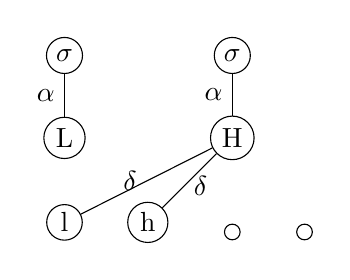
\begin{tikzpicture} [baseline = (y.base)]
\matrix (m) [matrix of nodes, column sep = 1.5em, row sep = 1.5em]{
\node[draw,circle, inner sep =2pt](x){$\sigma$}; & & \node[draw,circle, inner sep =2pt](x2){$\sigma$}; \\
\node[draw,circle, inner sep =2pt](y){L}; & & \node[draw,circle, inner sep =2pt](y2){H};  \\
\node[draw,circle, inner sep =2pt](z){l}; & \node[draw,circle, inner sep =2pt](v){h}; & \node[draw,circle, inner sep =2pt](z2){\hspace{1em}}; & \node[draw,circle, inner sep =2pt](v2){\hspace{1em}}; \\
};
\draw (x) -- (y) node[left, pos=.5]{$\alpha$};
\draw (z) -- (y2) node[left, pos=.5]{$\delta$};
\draw (v) -- (y2) node [right, pos =.4]{$\delta$};
\draw (x2) -- (y2) node[left, pos=.5]{$\alpha$};
\end{tikzpicture}
\end{center}
We have shown that contour spread \emph{can} be represented using Yip's tonal geometry. Additionally, we have defined the dominance function in the transduction such that the contour on the first syllable spreads in a \emph{unit-like} manner (by referring to the structural position of the `dominator' in the input, but not to its substance, i.e., low register). In other words, it is possible to spread contour without spreading register in Yip's model, in spite of the fact that register immediately dominates terminal nodes.\par
Another option is to do a Zhenhai transduction from a Yip model input to a Bao model output. As was the case in the general transduction, this will require a copy set of size two. We follow the convention of the general model by defining the TBU and tonal root nodes in the first copy set only (thereby allowing an identical definition of association), with register, `c', and terminal tonal nodes defined in the second copy set. This transduction is presented below:
\begin{equation}
\begin{aligned}
P_{\sigma}^{1}(x)&\myeq P_{\sigma}(x) & P_{\sigma}^{2}(x)&\myeq\mathtt{False} \\
P_{T}^{1}(x)&\myeq P_{rf}(x) & P_{T}^{2}(x)&\myeq\mathtt{False} \\
P_{c}^{1}(x)&\myeq \mathtt{False} & P_{c}^{2}(x)&\myeq P_{rf}(x)\land \neg last(x) \\
P_{-u}^{1}(x)&\myeq \mathtt{False} & P_{-u}^{2}(x)&\myeq P_{\sigma}(x)\land \neg last(x) \\
P_{+u}^{1}(x)&\myeq \mathtt{False} & P_{+u}^{2}(x)&\myeq P_{\sigma}(x)\land  last(x) \\
P_{l}^{1}(x)&\myeq \mathtt{False} & P_{l}^{2}(x)&\myeq P_{l}(x)\land \neg last(\delta(x)) \\
P_{h}^{1}(x)&\myeq \mathtt{False} & P_{h}^{2}(x)&\myeq P_{h}(x)\land \neg last(\delta(x)) \\
\alpha^{1,1}(x)=y&\myeq \alpha(x)=y & \alpha^{1,2}(x)=y&\myeq\mathtt{False} \\
\alpha^{2,1}(x)=y&\myeq \mathtt{False} & \alpha^{2,2}(x)=y&\myeq\mathtt{False} \\
\delta^{1,1}(x)=y&\myeq \mathtt{False} & \delta^{1,2}(x)=y&\myeq \mathtt{False} \\
\delta^{2,1}(x)=y&\myeq \Big[ P_{\sigma}(x)\land P_{rf}(y)\land & \delta^{2,2}(x)=y&\myeq \Big[ P_{l}(x)\land P_{rf}(y) \land \\
&\quad \, \, \neg last(x)\land \neg last(y)\Big]\lor & &\quad \, \, \neg last(\delta(x))\land \neg last(y)\Big] \lor \\
&\quad \, \, \Big[ P_{\sigma}(x)\land P_{rf}(y)\land & &\quad \, \, \Big[ P_{h}(x)\land P_{rf}(y)\land \\
&\quad \, \, last(x)\land last(y)\Big] \lor & &\quad \, \, \neg last(\delta(x))\land \neg last(y)\Big] \\
&\quad \, \, \Big[ P_{rf}(x)\land P_{rf}(y) \land \\
&\quad \, \, \neg last(x) \land last(y)\Big]
\end{aligned}
\end{equation}
Graphically, this transduction is:
\begin{center}
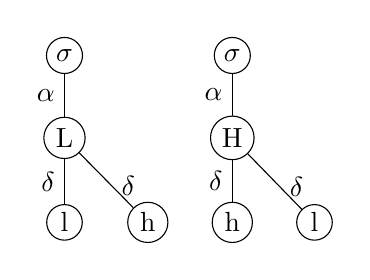
\begin{tikzpicture} [baseline = (y.base)]
\matrix (m) [matrix of nodes, column sep = 1.5em, row sep = 1.5em]{
\node[draw,circle, inner sep =2pt](x){$\sigma$}; & & \node[draw,circle, inner sep =2pt](x2){$\sigma$}; \\
\node[draw,circle, inner sep =2pt](y){L}; & & \node[draw,circle, inner sep =2pt](y2){H};  \\
\node[draw,circle, inner sep =2pt](z){l}; & \node[draw,circle, inner sep =2pt](v){h}; & \node[draw,circle, inner sep =2pt](z2){h}; & \node[draw,circle, inner sep =2pt](v2){l}; \\
};
\draw (x) -- (y) node[left, pos=.5]{$\alpha$};
\draw (z) -- (y) node[left, pos=.5]{$\delta$};
\draw (v) -- (y) node [right, pos =.4]{$\delta$};
\draw (x2) -- (y2) node[left, pos=.5]{$\alpha$};
\draw (z2) -- (y2) node[left, pos=.5]{$\delta$};
\draw (v2) -- (y2) node [right, pos =.4]{$\delta$};
\end{tikzpicture}
\hspace{.5cm}
$\rightarrow$
\hspace{.5cm}
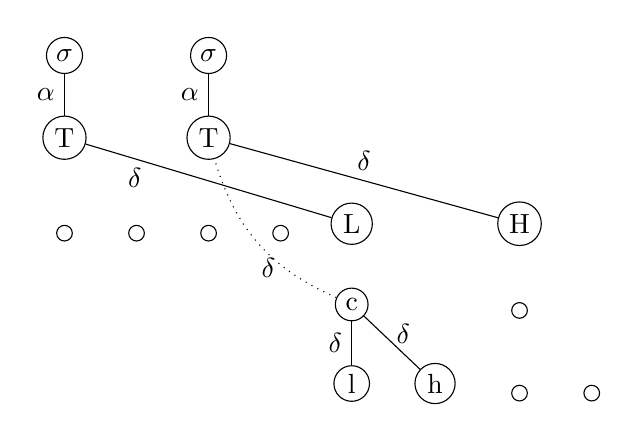
\begin{tikzpicture} [baseline = (y.base)]
\matrix (m) [matrix of nodes, column sep = 1.5em, row sep = 1.5em]{
\node[draw,circle, inner sep =2pt](x){$\sigma$}; & & \node[draw,circle, inner sep =2pt](x2){$\sigma$}; \\
\node[draw,circle, inner sep =2pt](y){T}; & & \node[draw,circle, inner sep =2pt](y2){T};  \\
\node[draw,circle, inner sep =2pt](z){\hspace{1em}}; & \node[draw,circle, inner sep =2pt](v){\hspace{1em}}; & \node[draw,circle, inner sep =2pt](z2){\hspace{1em}}; & \node[draw,circle, inner sep =2pt](v2){\hspace{1em}}; & \node[draw,circle, inner sep =2pt](x21){L}; & & \node[draw,circle, inner sep =2pt](x22){H};  \\
& & & & \node[draw,circle, inner sep =2pt](y21){c}; & & \node[draw,circle, inner sep =2pt](y22){\hspace{1em}}; \\
& & & & \node[draw,circle, inner sep =2pt](z21){l}; & \node[draw,circle, inner sep =2pt](v21){h}; & \node[draw,circle, inner sep =2pt](z22){\hspace{1em}}; & \node[draw,circle, inner sep =2pt](v22){\hspace{1em}}; \\
};
\draw (x) -- (y) node[left, pos=.5]{$\alpha$};
\draw (x2) -- (y2) node[left, pos=.5]{$\alpha$};
\draw (x21) -- (y) node [below, pos=.8]{$\delta$};
\draw (x22) -- (y2) node [above, pos=.5]{$\delta$};
\draw (z21) -- (y21) node [left, pos=.5]{$\delta$};
\draw (v21) -- (y21) node [above, pos=.3]{$\delta$};
\path [dotted] (y21) edge [bend left = 25] node[left, pos=.3]{$\delta$} (y2);
\end{tikzpicture}
\end{center}
\end{document}
